\documentclass[11pt,preprint, authoryear]{elsarticle}

\usepackage{lmodern}
%%%% My spacing
\usepackage{setspace}
\setstretch{1.2}
\DeclareMathSizes{12}{14}{10}{10}

% Wrap around which gives all figures included the [H] command, or places it "here". This can be tedious to code in Rmarkdown.
\usepackage{float}
\let\origfigure\figure
\let\endorigfigure\endfigure
\renewenvironment{figure}[1][2] {
    \expandafter\origfigure\expandafter[H]
} {
    \endorigfigure
}

\let\origtable\table
\let\endorigtable\endtable
\renewenvironment{table}[1][2] {
    \expandafter\origtable\expandafter[H]
} {
    \endorigtable
}


\usepackage{ifxetex,ifluatex}
\usepackage{fixltx2e} % provides \textsubscript
\ifnum 0\ifxetex 1\fi\ifluatex 1\fi=0 % if pdftex
  \usepackage[T1]{fontenc}
  \usepackage[utf8]{inputenc}
\else % if luatex or xelatex
  \ifxetex
    \usepackage{mathspec}
    \usepackage{xltxtra,xunicode}
  \else
    \usepackage{fontspec}
  \fi
  \defaultfontfeatures{Mapping=tex-text,Scale=MatchLowercase}
  \newcommand{\euro}{€}
\fi

\usepackage{amssymb, amsmath, amsthm, amsfonts}

\def\bibsection{\section*{References}} %%% Make "References" appear before bibliography


\usepackage[round]{natbib}

\usepackage{longtable}
\usepackage[margin=2.3cm,bottom=2cm,top=2.5cm, includefoot]{geometry}
\usepackage{fancyhdr}
\usepackage[bottom, hang, flushmargin]{footmisc}
\usepackage{graphicx}
\numberwithin{equation}{section}
\numberwithin{figure}{section}
\numberwithin{table}{section}
\setlength{\parindent}{0cm}
\setlength{\parskip}{1.3ex plus 0.5ex minus 0.3ex}
\usepackage{textcomp}
\renewcommand{\headrulewidth}{0pt}

\usepackage{array}
\newcolumntype{x}[1]{>{\centering\arraybackslash\hspace{0pt}}p{#1}}

%%%%  Remove the "preprint submitted to" part. Don't worry about this either, it just looks better without it:
\makeatletter
\def\ps@pprintTitle{%
  \let\@oddhead\@empty
  \let\@evenhead\@empty
  \let\@oddfoot\@empty
  \let\@evenfoot\@oddfoot
}
\makeatother

 \def\tightlist{} % This allows for subbullets!

\usepackage{hyperref}
\hypersetup{breaklinks=true,
            bookmarks=true,
            colorlinks=true,
            citecolor=blue,
            urlcolor=blue,
            linkcolor=blue,
            pdfborder={0 0 0}}


% The following packages allow huxtable to work:
\usepackage{siunitx}
\usepackage{multirow}
\usepackage{hhline}
\usepackage{calc}
\usepackage{tabularx}
\usepackage{booktabs}
\usepackage{caption}


\newenvironment{columns}[1][]{}{}

\newenvironment{column}[1]{\begin{minipage}{#1}\ignorespaces}{%
\end{minipage}
\ifhmode\unskip\fi
\aftergroup\useignorespacesandallpars}

\def\useignorespacesandallpars#1\ignorespaces\fi{%
#1\fi\ignorespacesandallpars}

\makeatletter
\def\ignorespacesandallpars{%
  \@ifnextchar\par
    {\expandafter\ignorespacesandallpars\@gobble}%
    {}%
}
\makeatother

\newenvironment{CSLReferences}[2]{%
}

\urlstyle{same}  % don't use monospace font for urls
\setlength{\parindent}{0pt}
\setlength{\parskip}{6pt plus 2pt minus 1pt}
\setlength{\emergencystretch}{3em}  % prevent overfull lines
\setcounter{secnumdepth}{5}

%%% Use protect on footnotes to avoid problems with footnotes in titles
\let\rmarkdownfootnote\footnote%
\def\footnote{\protect\rmarkdownfootnote}
\IfFileExists{upquote.sty}{\usepackage{upquote}}{}

%%% Include extra packages specified by user

%%% Hard setting column skips for reports - this ensures greater consistency and control over the length settings in the document.
%% page layout
%% paragraphs
\setlength{\baselineskip}{12pt plus 0pt minus 0pt}
\setlength{\parskip}{12pt plus 0pt minus 0pt}
\setlength{\parindent}{0pt plus 0pt minus 0pt}
%% floats
\setlength{\floatsep}{12pt plus 0 pt minus 0pt}
\setlength{\textfloatsep}{20pt plus 0pt minus 0pt}
\setlength{\intextsep}{14pt plus 0pt minus 0pt}
\setlength{\dbltextfloatsep}{20pt plus 0pt minus 0pt}
\setlength{\dblfloatsep}{14pt plus 0pt minus 0pt}
%% maths
\setlength{\abovedisplayskip}{12pt plus 0pt minus 0pt}
\setlength{\belowdisplayskip}{12pt plus 0pt minus 0pt}
%% lists
\setlength{\topsep}{10pt plus 0pt minus 0pt}
\setlength{\partopsep}{3pt plus 0pt minus 0pt}
\setlength{\itemsep}{5pt plus 0pt minus 0pt}
\setlength{\labelsep}{8mm plus 0mm minus 0mm}
\setlength{\parsep}{\the\parskip}
\setlength{\listparindent}{\the\parindent}
%% verbatim
\setlength{\fboxsep}{5pt plus 0pt minus 0pt}



\begin{document}



\begin{frontmatter}  %

\title{COVID-19}

% Set to FALSE if wanting to remove title (for submission)




\author[Add1]{Hannah MacGinty}
\ead{21082022@sun.ac.za}





\address[Add1]{Stellenbosch, South Africa}


\begin{abstract}
\small{
This report analyses the global and country-specific trends associated
with the COVID-19 pandemic.
}
\end{abstract}

\vspace{1cm}





\vspace{0.5cm}

\end{frontmatter}

\setcounter{footnote}{0}



%________________________
% Header and Footers
%%%%%%%%%%%%%%%%%%%%%%%%%%%%%%%%%
\pagestyle{fancy}
\chead{}
\rhead{}
\lfoot{}
\rfoot{}
\lhead{}
%\rfoot{\footnotesize Page \thepage } % "e.g. Page 2"
\cfoot{}

%\setlength\headheight{30pt}
%%%%%%%%%%%%%%%%%%%%%%%%%%%%%%%%%
%________________________

\headsep 35pt % So that header does not go over title




\hypertarget{introduction}{%
\section{\texorpdfstring{Introduction
\label{Introduction}}{Introduction }}\label{introduction}}

I have been tasked to examine the evolution of the Covid-19 outbreak.

\hypertarget{data}{%
\section*{Data}\label{data}}
\addcontentsline{toc}{section}{Data}

The data looks at Covid-19 globally.

\hypertarget{experience-of-african-countries}{%
\subsection{Experience of African
Countries}\label{experience-of-african-countries}}

I provide insights into how African countries experienced the COVID-19
pandemic compared to other regions.

First, the average total cases for Africa is plotted over time. They
steeply rose over time. The next figure compares Africa across
continents. It had the lowest increase (flattest slope) in COVID cases
over time. Europe, on the other hand, faced rapid increases in COVID-19,
rising particularly steeply throughout.

Africa also has the least fully vaccinated people per hundred people.
This is possibly due to being under-resourced. Oceana, mostly comprising
Australia, has the highest population of fully vaccinated people.

\begin{figure}[H]

{\centering \includegraphics{Q1_files/figure-latex/Figure1-1} 

}

\caption{COVID-19 Cases per Million \label{Figure1}}\label{fig:Figure1-1}
\end{figure}
\begin{figure}[H]

{\centering \includegraphics{Q1_files/figure-latex/Figure1-2} 

}

\caption{COVID-19 Cases per Million \label{Figure1}}\label{fig:Figure1-2}
\end{figure}
\begin{figure}[H]

{\centering \includegraphics{Q1_files/figure-latex/Figure1-3} 

}

\caption{COVID-19 Cases per Million \label{Figure1}}\label{fig:Figure1-3}
\end{figure}

\hypertarget{severity-of-covid-19-in-countries-with-high-vs-low-life-expectancy}{%
\subsection{Severity of COVID-19 in Countries with High vs Low Life
Expectancy}\label{severity-of-covid-19-in-countries-with-high-vs-low-life-expectancy}}

Next I want to examine distinct patterns in the severity of their COVID
experience in countries with higher and lower general life expectancy.
By averaging life expectancy across locations, the five countries with
the lowest life expectancy are Central African Republic, Chad, Lesotho,
Nigeria and Sierra Leone.

From the below tables, we can see that Africa has the lowest Life
Expectancy and Europe has the highest.

Among countries with the lowest life expectancy, total deaths remained
relatively low except for Nigeria, where deaths roses rapidly from the
beginning of 2020 to the end of 2022. Lesotho experienced the next
highest number of deaths.

The five countries/locations with the highest life expectancies were
Monaco (86.8 years), San Marino, Hong Kong, Japan, and Macao. Among
countries with the highest life expectancy, Japan had the highest number
of deaths, reaching over 30 000 around quarter 3 of 2022. Deaths were
very low in the locations of Monaco, San Marino, and Macao.

\begin{figure}[H]

{\centering 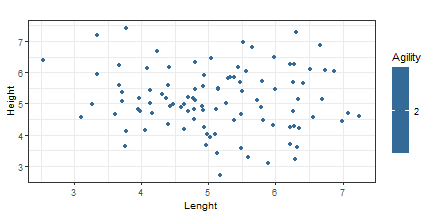
\includegraphics{Q1_files/figure-latex/Figure2-1} 

}

\caption{Caption Here \label{Figure2}}\label{fig:Figure2-1}
\end{figure}
\begin{figure}[H]

{\centering 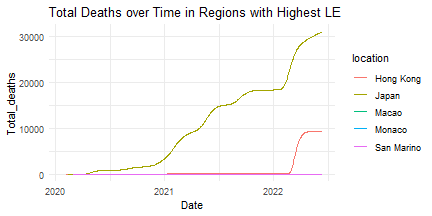
\includegraphics{Q1_files/figure-latex/Figure2-2} 

}

\caption{Caption Here \label{Figure2}}\label{fig:Figure2-2}
\end{figure}

Total cases per million where the highest in Lesotho, probably owing to
its small population. For areas with high life expectancy, San Marino
experienced the highest number of cases per million people, followed by
Macao.

\begin{figure}[H]

{\centering 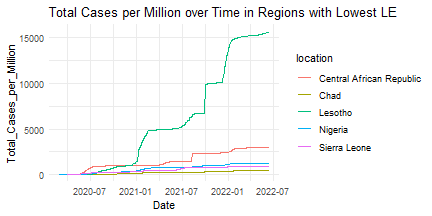
\includegraphics{Q1_files/figure-latex/Figure3-1} 

}

\caption{Caption Here \label{Figure3}}\label{fig:Figure3-1}
\end{figure}
\begin{figure}[H]

{\centering 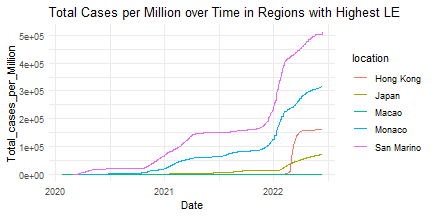
\includegraphics{Q1_files/figure-latex/Figure3-2} 

}

\caption{Caption Here \label{Figure3}}\label{fig:Figure3-2}
\end{figure}

\hypertarget{changes-in-general-and-icu-hospitalisation}{%
\subsection{Changes in General and ICU
Hospitalisation}\label{changes-in-general-and-icu-hospitalisation}}

Hospitalisations and ICU admissions are plotted.

Plotting across continent, we can see that each continent experienced
waves of hospitalisation at different times. Europe, North America and
Asia experienced the highest shocks in hospitalisations.
Hospitalisations in Africa were always low. This is expected given the
cases were fewer.

\begin{figure}[H]

{\centering 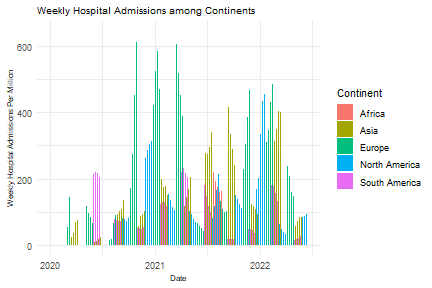
\includegraphics{Q1_files/figure-latex/Figure4-1} 

}

\caption{Hospital Admissions \label{Figure4}}\label{fig:Figure4}
\end{figure}

Europe and South America experienced the highest numbers of weekly ICU
admission per million . This is interesting because South America did
not have as sharp spikes in general hospitalisations compared to other
continents.

\begin{figure}[H]

{\centering 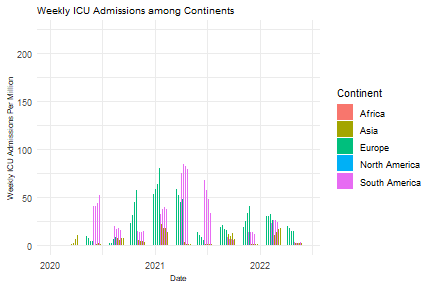
\includegraphics{Q1_files/figure-latex/Figure5-1} 

}

\caption{Hospital Admissions \label{Figure5}}\label{fig:Figure5}
\end{figure}

Plotting hospital patients and ICU patients, it can be seen that they
follow the same trends and waves. ICU patient numbers always increase
globally when global hospitalisations increase. Therefore, general
hospitalisation led ICU hospitalisations.

We can also see that there is a positive correlation (0.6) between the
numberr of hospital patients and number of tests. Therefore, the number
of tests conducted can act as a good indicator of hospitalisation.

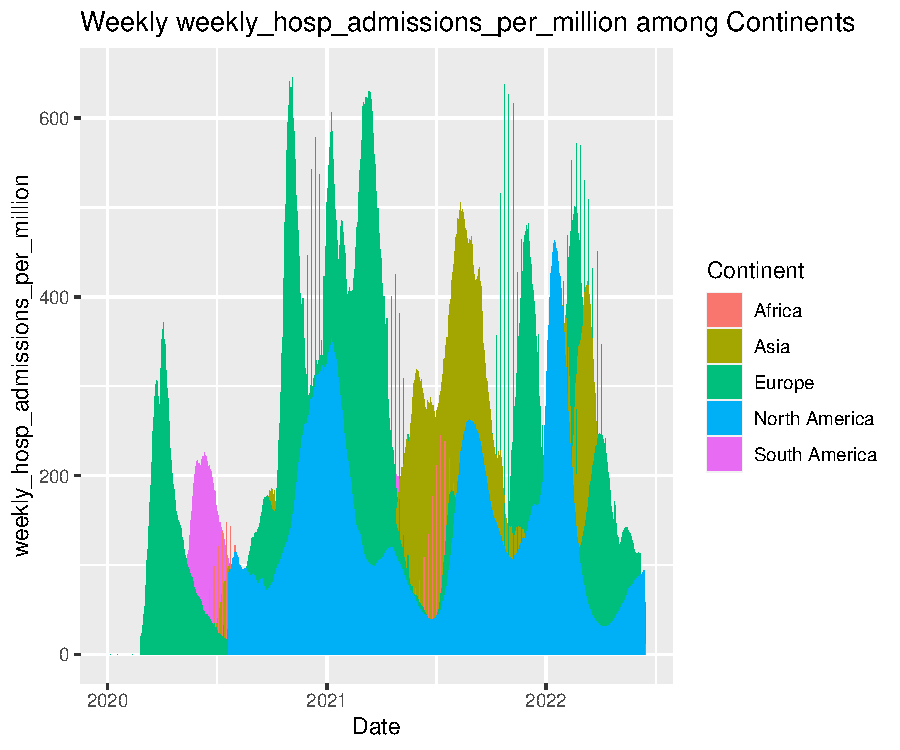
\includegraphics{Q1_files/figure-latex/unnamed-chunk-2-1.pdf}

\begin{verbatim}
## [1] 0.6159445
\end{verbatim}

In South Africa, there are clear waves in hospitalisations. This shows
how hospitalisations were clustered mostly likely when during times when
the virus spread was high.

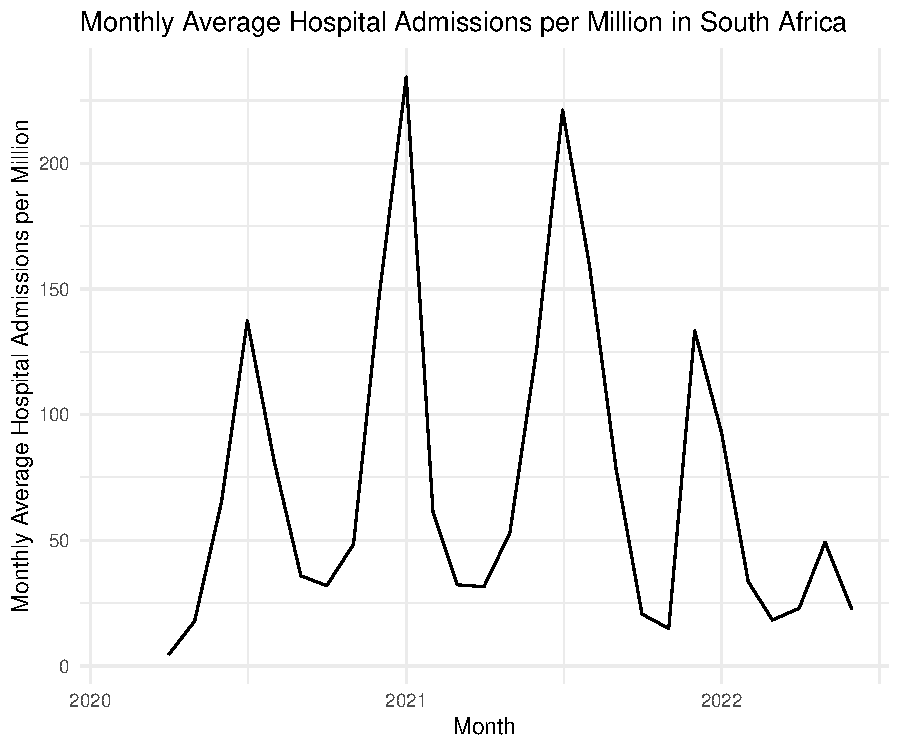
\includegraphics{Q1_files/figure-latex/unnamed-chunk-3-1.pdf}

\hfill

\hypertarget{discussion-and-conclusion}{%
\section*{Discussion and Conclusion}\label{discussion-and-conclusion}}
\addcontentsline{toc}{section}{Discussion and Conclusion}

In conclusion, Covid-19 wrecked havoc throughout the world, leading to
increase deaths and hospitalisations. Africa experienced less COVID-19
cases compared to the rest of the world and consequently, less deaths.
This could also be due to a lack of proper recording of COVID data.

By looking at countries with different life expectancies, the results
are mixed. Total deaths were high and approximately the same in Japan
and Nigeria, despite having very different life expectancies. Deaths
were relatively low in the other specified areas. Total cases per
million were typically higher in countries with high life expectancy. By
not having substantially higher deaths in these countries, it is likely
that citizens in high life expectancy countries had strong enough immune
systems to cope with the virus.

It is clear that COVID presented itself in waves and these waves
impacted different continents at different times. ICU hospitalisations
were strongly associated with Hospital admissions.

\newpage

\bibliography{Tex/ref}





\end{document}
